\chapter{Materials and Methods}

\section{Motion Segmentation }
As reported in D9, we developed a novel motion segmentation algorithm utilizing neuromorphic vision sensor. The algorithm was characterized by experiments in controlled environments. The paper has been submitted to Frontiers in Neuroscience. The next step was to integrate the algorithm with a virtual reality platform, allowing a controller to remotely visualize the environment and interact with the robot.
\begin{figure}[h!]
  \begin{center}
    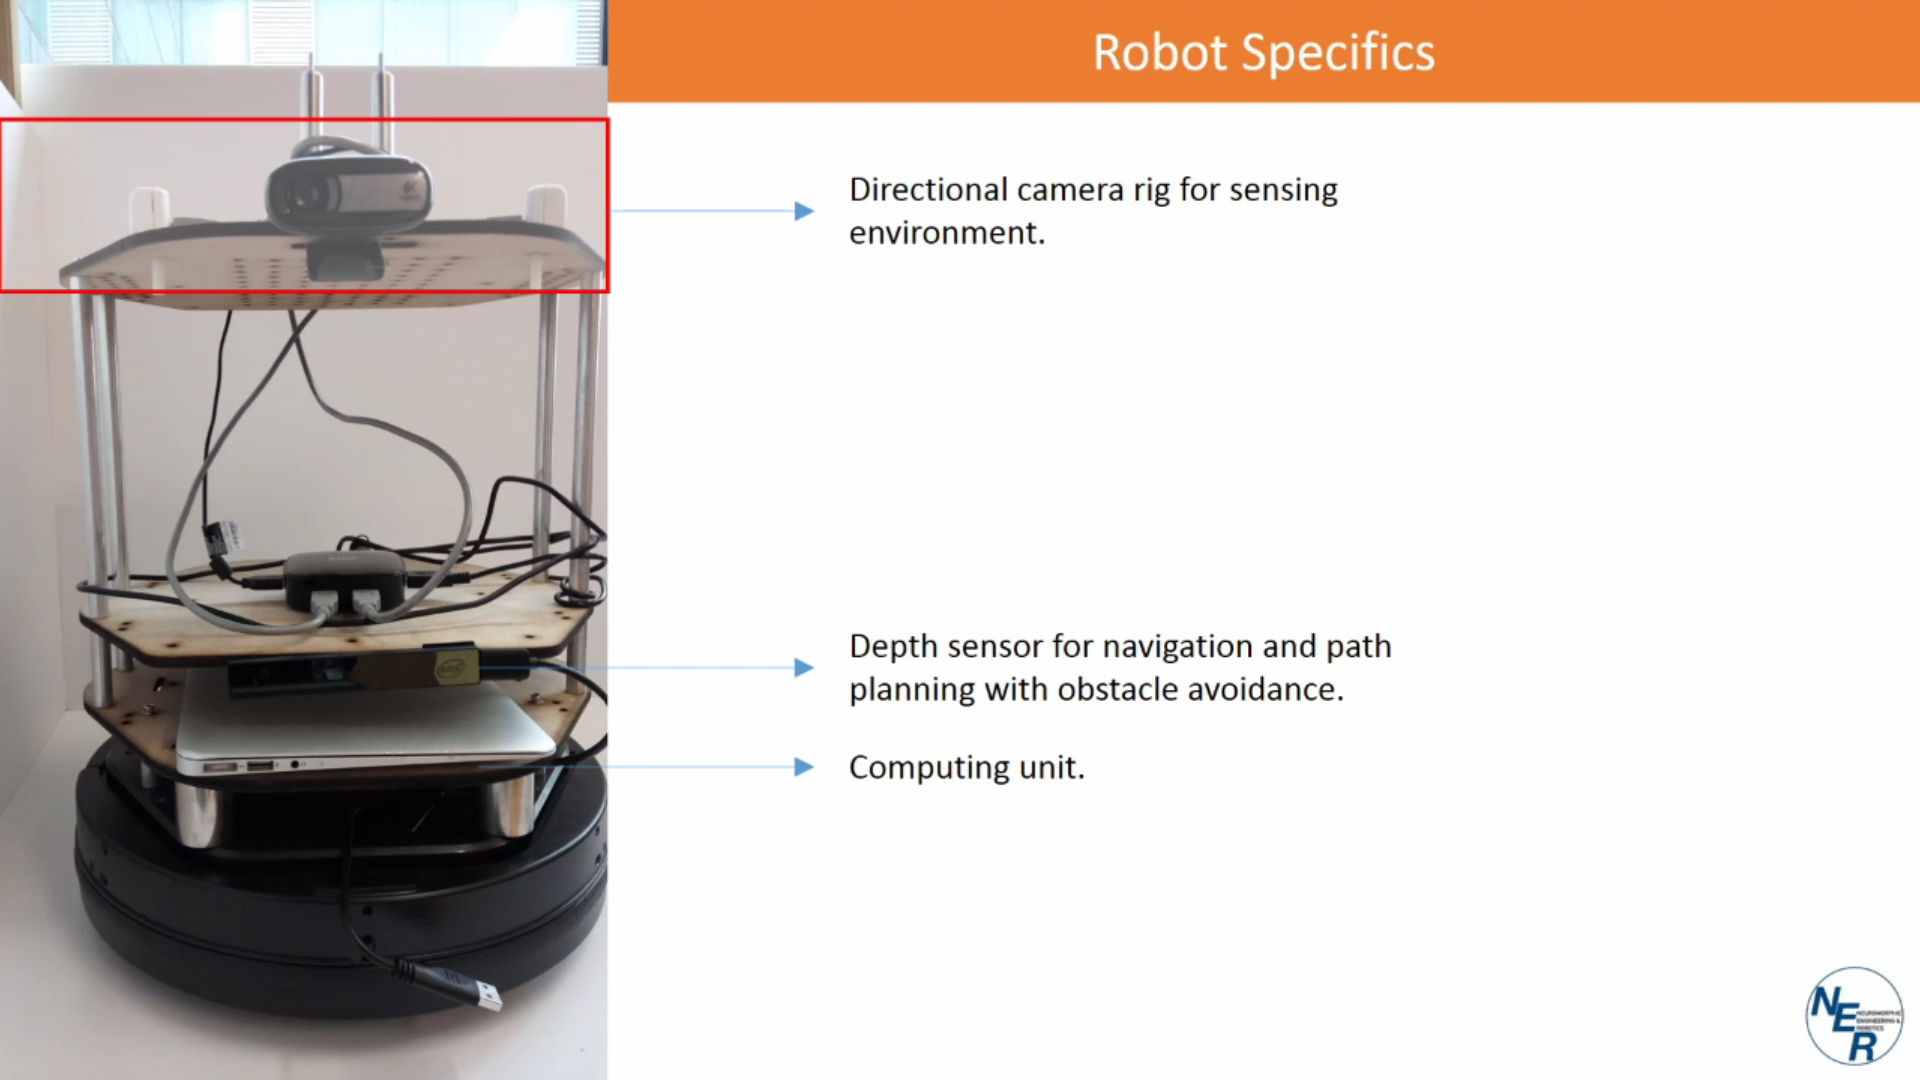
\includegraphics[width=0.90\textwidth]{figures/motion-seg/setup}% This is a *.jpg file
  \end{center}
  \textbf{\refstepcounter{figure}\label{fig:turtle_setup} Figure \arabic{figure}. Sensor integration in the robotic platform for experiments.} { The robot is ROS-enabled and allows development of algorithms within the ROS ecosystem. }
\end{figure}

In this report, we emphasize on the development of (1) the robotic platform for integrating various sensors for navigation and motion segmentation and (2) wireless data transfer and rendition in a virtual reality platform. As shown in Fig\ref{fig:turtle_setup}, we use the turtlebot robotic platform to integrate the sensors and algorithms. The robot comprises three USB cameras with their field of views (FoV) aligned such that they form a continuous scene when rendered consecutively. The robot is equipped with a RGBD sensor, Intel's RealSense R200, allowing the robot to make a map of its environment and perform path planning. A central computing unit is responsible for executing the algorithms for path planning, obstacle avoidance, motion segmentation and wireless environment image transfer.

Fig\ref{fig:VR_setup} shows the corresponding data as received by the virtual reality platform. The current implementation uses image data encoded as a motion-JPEG (mjpg) video stream at $20fps$, rendered by a viewer such as a web browser. The robot is located in a remote location and implements the algorithms for navigation, path planning and obstacle avoidance.
\begin{figure}[h!]
  \begin{center}
    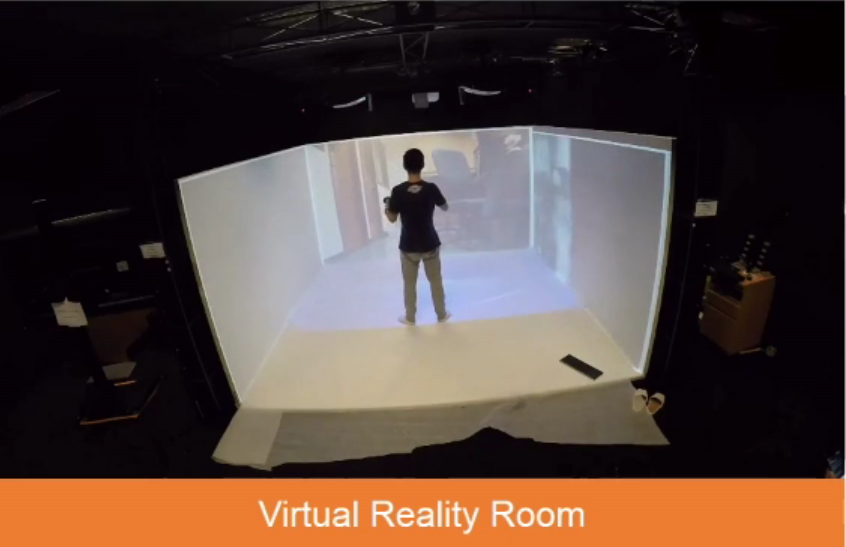
\includegraphics[width=0.90\textwidth]{figures/motion-seg/VR-Robot}% This is a *.jpg file
  \end{center}
  \textbf{\refstepcounter{figure}\label{fig:VR_setup} Figure \arabic{figure}. Rendition of data from the robot.} { Data from the three directional cameras installed on the robot is displayed in the virtual reality platform. }
\end{figure}

Fig\ref{fig:robot-env}(A) shows the 2D map that is calculated and stored locally on the robot's computing unit for navigation and obstacle avoidance. The arrow indicates the location of the robot in the map with the corresponding physical location as shown in Fig\ref{fig:robot-env}(B). A gesture tracking algorithm was developed that manipulates robot's motion parameters in real-time.
\begin{figure}[h!]
  \begin{center}
    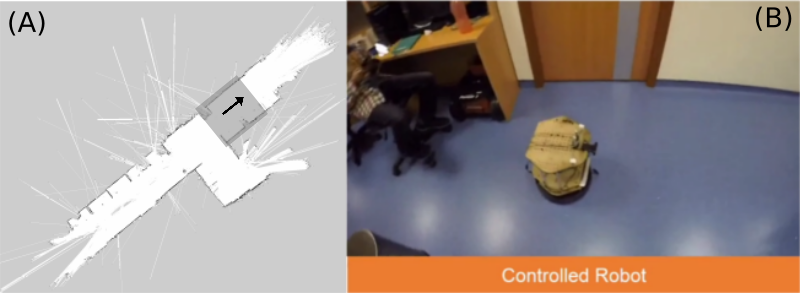
\includegraphics[width=0.95\textwidth]{figures/motion-seg/robot-env}% This is a *.jpg file
  \end{center}
  \textbf{\refstepcounter{figure}\label{fig:robot-env} Figure \arabic{figure}. Robot's map and physical location.} { (A) A 2D map created using the RGBD sensor is shown. (B) The corresponding physical location of the robot is shown. }
\end{figure}

\section{Vibro-Tactile Haptic Glove}

As reported in D9 report, we developed the second generation
vibro-tactile gloves with flexible PCB to reduce wiring. However due
to the stiffness of the PCB and the dissipation of vibro-tactile
stimuli on the palm region experienced by the user, we developed third
generation of vibrotactile glove. In this version, we use wires to
fasten the actuators and give the user a more natural feel.

In the third-generation, eighteen actuators are placed at sensitive
locations of human’s hand~Fig\ref{fig:glove}. This generation of haptic glove is flexible
and light weight.

\begin{figure}[!ht]
  \centering
  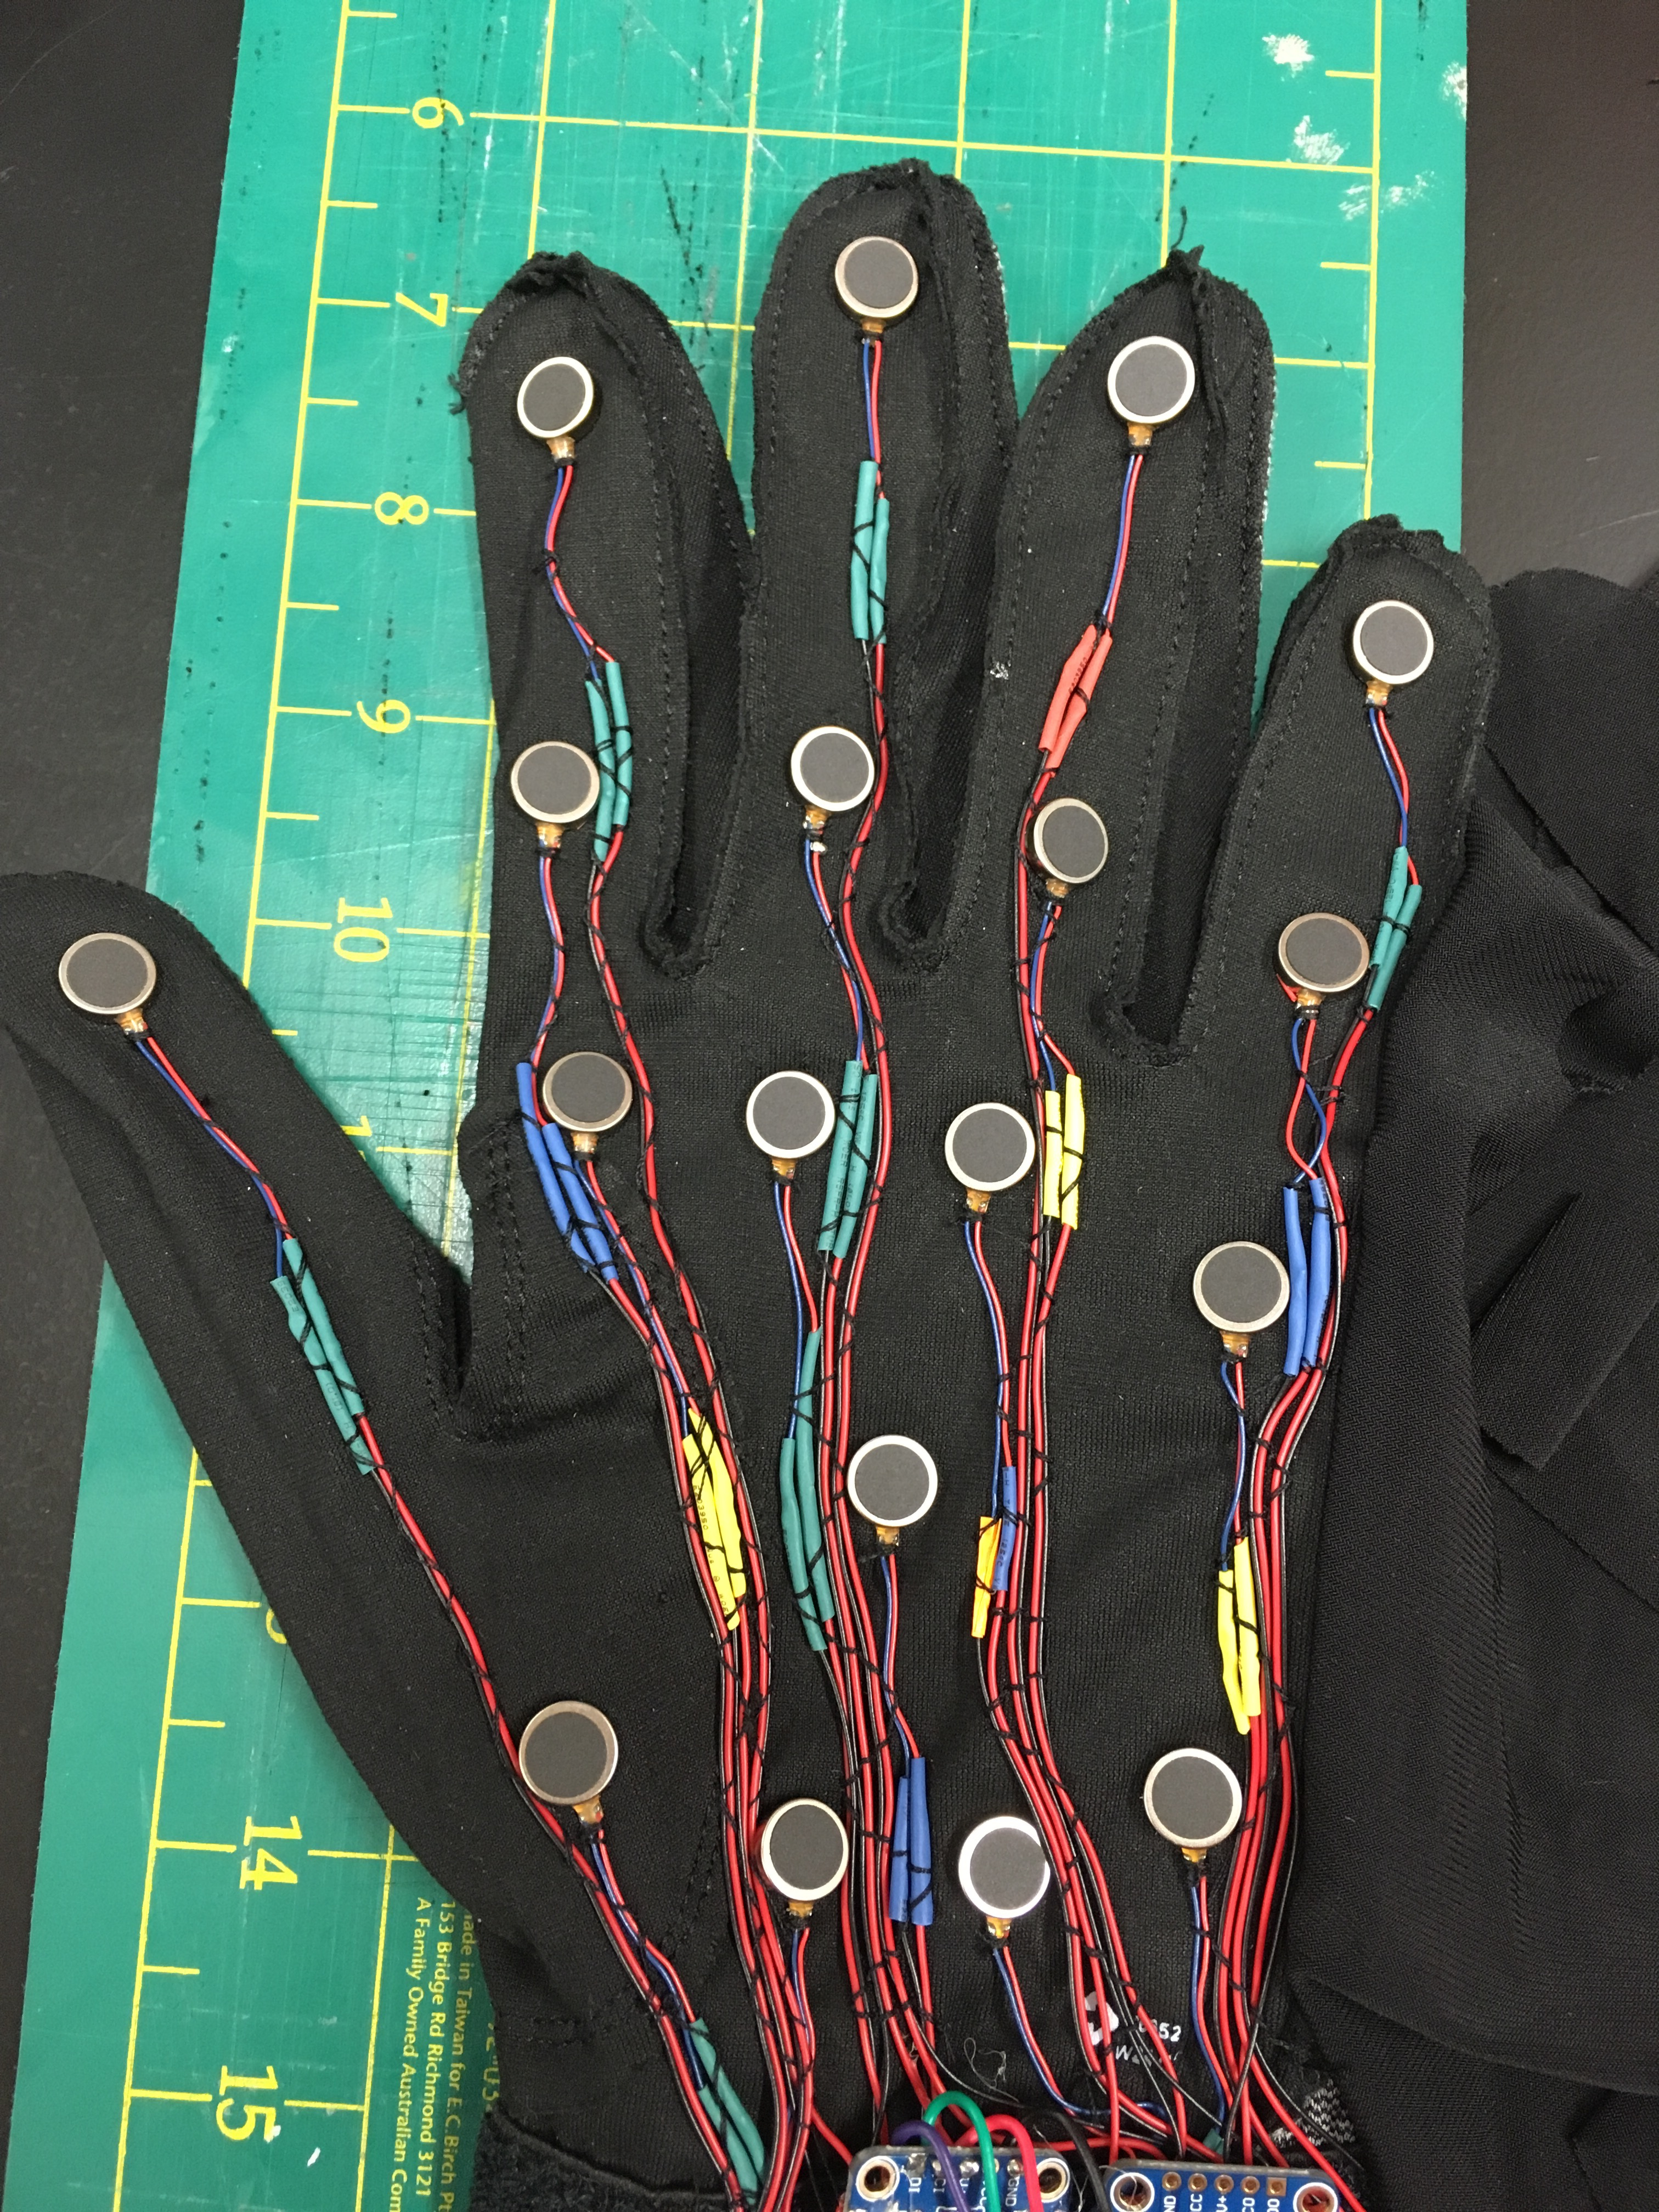
\includegraphics[width=5cm]{figures/figure1.jpg}
  \caption{Third Generation Vibrotactile Gloves.}
  \label{fig:glove}
\end{figure}

The glove is controlled by pulse width modulation (PWM) drivers and arduino microcontroller. As shown in~Fig\ref{fig:glove}, PWM drivers, arduino microcontroller and battery to drive the circuit, is housed in the control box.

\begin{figure}[!ht]
  \centering
  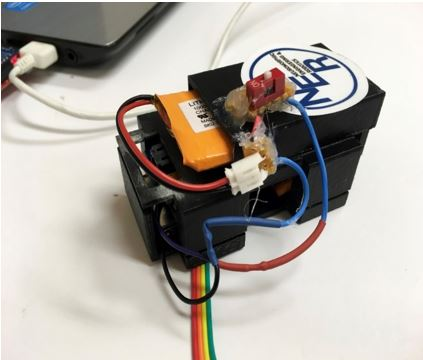
\includegraphics[width=8cm]{figures/figure2.jpg}
  \caption{Control Box Housing.}
  \label{fig:box}
\end{figure}


Fig\ref{fig:glove-gui} displays the connection between haptic glove and control
box. We have developed a graphical user interface to enable single and
multiple actuator activation. The intensity of each actuators is
controlled by the corresponding slider.  (Figure 4).

\begin{figure}[!ht]
  \centering
  \subfigure[Control Box Connection.]{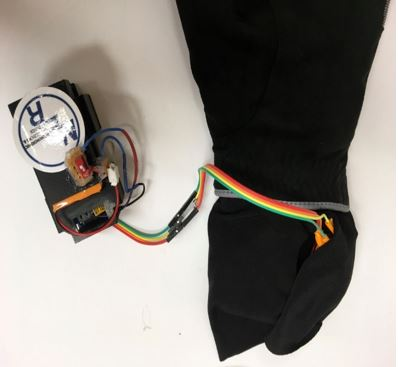
\includegraphics[height = 2in]{figures/figure3.jpg}}
  \subfigure[GUI to Control Individual
  Actuators. ]{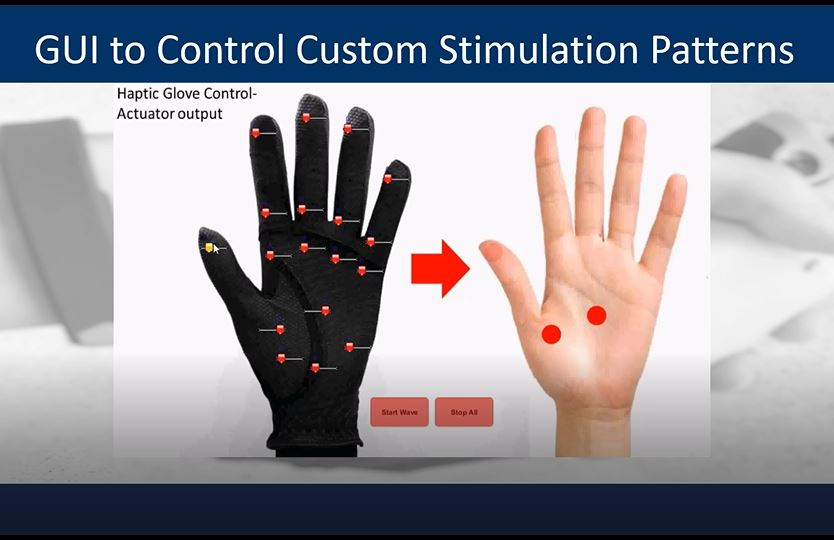
\includegraphics[height = 2in]{figures/figure4.jpg}}
  \caption{Haptic Glove Control Box and GUI Software.}
  \label{fig:glove-gui}
\end{figure}

The communication pathway is initiated by transmitting an encoded stimulation signal generated by the Graphical user interface at the computer terminal. It is received by the control box connected with the glove. This signal controls the vibration intensity of the actuators. As illustrated in Fig\ref{fig:gui-code}, the microcontroller is programmed to work with five voltage amplitudes. 

\begin{figure}[!ht]
  \centering
  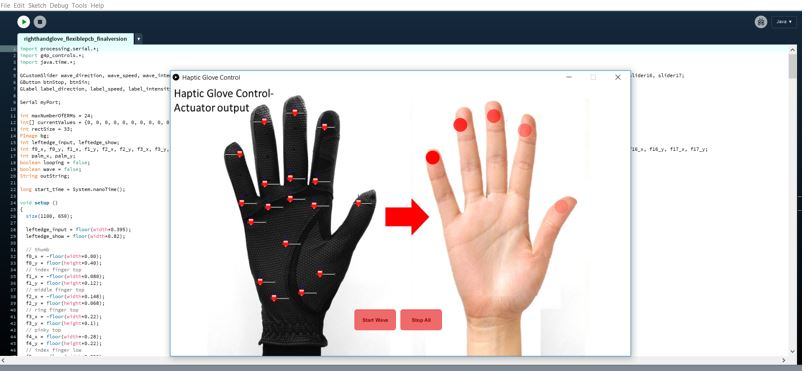
\includegraphics[width=9cm]{figures/figure5.jpg}
  \caption{GUI Displaying Different Amplitude Intensity Levels.}
  \label{fig:gui-code}
\end{figure}


\section{CAVE VR}

We aim at rendering complex virtual objects as shown in Figure 2, to
the user by mapping their shapes to the vibratory stimuli on the
haptic glove.

Based on the previous development. We designed gesture language
systems based on ART D-Track markers. %% add citation here for design
%% framework of 3d gestures
We conducted basic analysis on VR tasks and gesture segmentation, and
selected HMM as one of the core models for the system
design. 


The VR environment we built contains different
scenes. Each scene comes with  a set of gesture time sequence design
requirements that are vital for the completion of the task. Further
work will provide the implementation of the algorithmic architecture.  

Fig\ref{fig:pickplace} shows a scene for a simple pick and
place task. This scene requires non consistent gesture signal(pick and
drop). 

\begin{figure}[!ht]
  \centering
  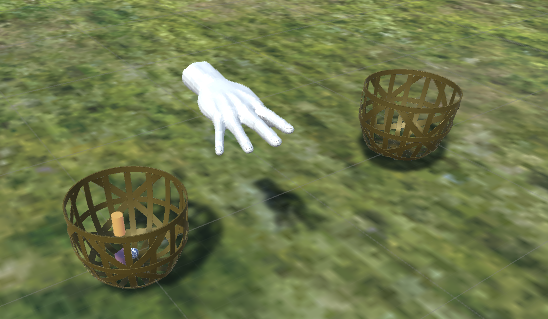
\includegraphics[width=8cm]{figures/pickplace.png}
  \caption{Pick and Place Task Scene}
  \label{fig:pickplace}
\end{figure}

